\capitulo{3}{Conceptos teóricos}

Se sintetizarán a continuación algunos de los conceptos teóricos más relevantes para la correcta comprensión del documento.

\section{Apendizaje automático}

Se denomina aprendizaje automático a aquella rama de la inteligencia artificial cuyo objetivo es desarrollar métodos que permitan que un algoritmo mejore su rendimiento mediante la experiencia y procesado de datos. Consecuentemente, los modelos entrenados realizarán predicciones cada vez más precisas como resultado del algoritmo implementado.

Dentro del aprendizaje automático se diferencian tres grandes grupos en función del tipo de entrada que sea consumida: el aprendizaje supervisado (datos etiquetados), el no supervisado (datos no etiquetados) y el semisupervisado (datos etiquetados y no etiquetados), siendo esta última categoría objeto de estudio en este proyecto de investigación. 

\section{Aprendizaje semisupervisado}

Como se ha mencionado anteriormente, se denomina aprendizaje semisupervisado a aquel conjunto de algoritmos que utiliza datos etiquetados y no etiquetados para realizar tareas de aprendizaje. Inicialmente, se pueden diferenciar dos categorías~\cite{engelen2020surveyOnSemiSupervised}: los métodos inductivos, cuyo objetivo principal es construir un clasificador que genere predicciones para cualquier entrada y los métodos transductivos, cuyo poder de predicción está limitado a los objetos utilizados en la fase de entrenamiento.


\begin{figure}[h]
\caption{Taxonomía de métodos de aprendizaje semisupervisados. Extraída de \textit{A survey on semi-supervised learning}~\cite{engelen2020surveyOnSemiSupervised}.}
\centering
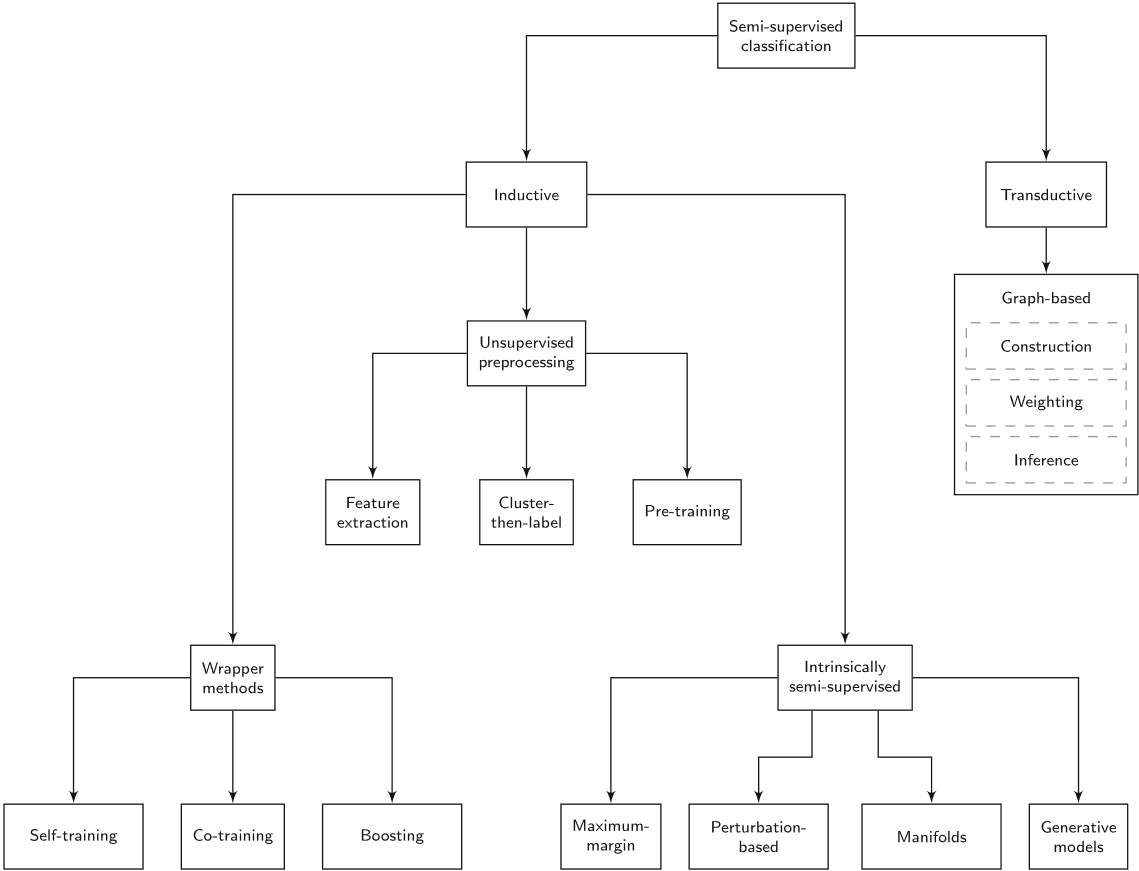
\includegraphics[width=\textwidth]{../img/memoria/esquemaHoos}
\end{figure}

Prescindiendo de los métodos transductivos por ser menos versátiles y útiles en nuestro propósito, los métodos inductivos se subdividen en tres grupos~\cite{engelen2020surveyOnSemiSupervised}: \textit{wrapper methods} (o métodos de envoltura), \textit{unsupervised preprocessing} y \textit{intrinsically semi-supervised}, siendo materia de estudio los métodos de envoltura. 


\subsection{Métodos de envoltura}

Estos modelos utilizan uno o más clasificadores que son entrenados iterativamente con los datos etiquetados de entrada, además de con datos pseudo-etiquetados. Se denomina pseudo-etiquetado a aquellos datos que inicialmente no estaban etiquetados, pero acabaron estándolo por iteraciones previas de los clasificadores.

Consecuentemente, el procedimiento consta de dos fases que se repiten en cada iteración: el entrenamiento y el pseudo-etiquetado. Durante el entrenamiento, los clasificadores se alimentan de datos etiquetados (o pseudo-etiquetados). En la fase de pseudo-etiquetado, se utilizan datos no etiquetados para que sean procesados por los clasificadores previamente entrenados. 

Dentro de esta categoría, se pueden diferenciar tres grandes grupos: \textit{self-training}, que utilizan únicamente un clasificador, \textit{co-training}~\cite{engelen2020surveyOnSemiSupervised}, que utilizan más de uno y los \textit{pseudo-labelled boosting methods}, que construyen clasificadores individuales que se alimentan de las predicciones más fiables. Se estudiará más en profundidad los métodos \textit{co-training}.

\subsubsection{Co-training}

En estos algoritmos, varios clasificadores son entrenados iterativamente utilizando datos etiquetados y añadiendo las predicciones (resultados) más confiables al conjunto para ser utilizadas en las siguientes iteraciones~\cite{engelen2020surveyOnSemiSupervised}. Para que los clasificadores sean capaces de generar información distinta, generalmente se divide el conjunto de entrada según alguna característica (no siendo estrictamente necesario). El \textit{co-forest}, algoritmo protagonista de este proyecto, pertenece a esta categoría.

TO-DO: Añadir información sobre las dos vistas independientes del co-training (otros métodos no tienen esta limitación)


\section{\textit{Ensembles}}

Se define \textit{ensemble} como un conjunto de modelos de \textit{machine learning} donde cada estimador base genera una predicción individual que se combina con el resto para generar una salida única~\cite{originalCoForest2007}. Los \textit{ensembles} pueden ser de clasificación o regresión, siendo los mostrados a continuación los más comunes.
	
\subsubsection{\textit{Bagging}}

Este modelo se compone de un conjunto de estimadores base entrenados en paralelo. Por lo tanto, el resultado es el promedio (o más popular) de las salidas de los modelos simples. Para entrenar cada estimador base se utiliza \textit{bootstrapping}~\cite{engelen2018thesis}, que es una técnica de muestreo que genera un subconjunto de datos seleccionando aleatoriamente muestras de un conjunto mayor permitiendo la repetición. Es decir, los clasificadores son entrenados con un subconjunto aleatorio del total de los datos etiquetados como se ilustra en la figura~\ref{img:bagging}.

\begin{figure}[h]
	\caption{Representación genérica de un modelo \textit{bagging}.}
	\label{img:bagging}
	\centering
	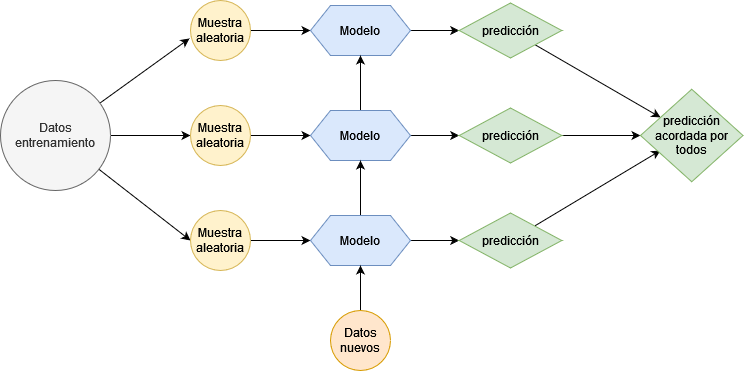
\includegraphics[width=\textwidth]{../img/memoria/bagging}
\end{figure}

\subsubsection{\textit{Random forest}}

Es uno de los métodos de \textit{bagging} más populares, que obtiene resultados certeros debido a la aleatoriedad introducida~\cite{originalCoForest2007}. Cuando se devuelve una etiqueta, es el resultado de una votación realizada por todos los árboles del conjunto. Además de utilizar \textit{bootstrapping}, en el entrenamiento individual de cada árbol, únicamente se <<ven>> algunos atributos (no el total) para introducir mayor aleatoriedad. Es decir, en cada nodo del árbol solo se tienen en cuenta ciertas características seleccionadas aleatoriamente.
	
\subsubsection{\textit{Boosting}}

Si el anterior modelo utiliza los clasificadores base <<en paralelo>>, este lo haría <<en serie>>~\cite{engelen2018thesis}. Es decir, hay un orden secuencial: los estimadores dependen del resultado anterior y tratan de compensar el error que se haya podido cometer.

El entrenamiento gira, por lo tanto, en torno a las instancias que hayan fallado los clasificadores previos. Esto es conseguido dando más peso a aquellas muestras mal clasificadas (en problemas de regresión, por ejemplo, las predicciones con un mayor error cuadrático medio tendrán más peso para el siguiente modelo). 


\section{\textit{Co-forest}}

\subsection{Descripción}

El denominado \textit{co-forest}~\cite{originalCoForest2007} es un método clasificador de aprendizaje semisupervisado (más concretamente, de envoltura) que permite construir un \textit{ensemble} de árboles de decisión. Este método está basado en el \textit{random forest} y se podría considerar su <<versión semisupervisada>>. 

Que sea un algoritmo semisupervisado implica que, durante la fase de entrenamiento, además de utilizar el conjunto de datos etiquetados ($L$), se utilicen también aquellas pseudo-etiquetas de las predicciones con mejor confianza del conjunto de datos no etiquetados ($U$).

El proceso de entrenamiento se realiza iterativamente~\cite{engelen2018thesis}, y en cada una de estas repeticiones, se examina cada árbol y se entrena individualmente con un subconjunto de $L$ ($L_{i}$) y con un subconjunto de $U$ ($L'_{i,t}$) formado por aquellas pseudo-etiquetas que, además de pertenecer a la submuestra (aleatoria), posean un nivel de confianza superior a un umbral definido por el usuario ($\theta$). Quienes estiman esta confianza de predicción para las muestras seleccionadas son el conjunto de todos los árboles que forman el \textit{ensemble} menos el árbol que está siendo entrenado individualmente (de ahora en adelante \textit{concomitant ensemble} o conjunto concomitante).

El criterio de parada de la fase de entrenamiento del \textit{co-forest} es el \textit{out-of-bag error}~\cite{zhou2021SemisupervisedRecommendationAttack} (de ahora en adelante, OOBE). Se define OOBE como el error que comete el conjunto concomitante de un árbol para el total de los datos etiquetados. Es decir, el número de árboles que aciertan la etiqueta entre el número de árboles que votan teniendo en cuenta que, para calcular el OOBE del total de los datos etiquetados, sólo votan aquellos árboles que no hayan utilizado la muestra concreta de $L$ para su entrenamiento.


\subsection{Algoritmo}


\subsubsection{Variables utilizadas}

Para facilitar la comprensión del pseudocódigo, se definen a continuación algunas de las variables utilizadas:
\begin{itemize}
	\item $n$: número total de árboles del ensemble.
	\item $h_{i}$: árbol i-ésimo del conjunto.
	\item $H_{i}$: \textit{concomitant ensemble} o conjunto concomitante del árbol i-ésimo (todos los árboles del \textit{co-forest} menos él).
	\item $x_j$: muestra j-ésima (generalmente sin etiqueta).
	\item $H_i(x_j)$: etiqueta asignada por $H_i$ a la muestra j-ésima.
	\item $w_{i,t,j}$: confianza de predicción (individual) calculada para una muestra $x_j$ por $H_{i}$ en la iteración $t$. Se define confianza como el grado de acuerdo que existe en una votación. 
	\item $W$: sumatorio de las confianzas de predicción individuales de un conjunto $W = \sum w_{i,t,j}$.
	\item $L$: conjunto de datos etiquetados utilizados durante el entrenamiento.
	\item $L_{i}$: subconjunto obtenido tras aplicar \textit{bootstrapping} a $L$ que se utiliza para entrenar el árbol $h_{i}$.
	\item $U$: conjunto de datos no etiquetados utilizados durante el entrenamiento.
	\item $U'_{i,t}$: subconjunto aleatorio de U cuya $W$ es menor que $Wmax$ (consultar ecuación~\ref{eqn:Wmax}).
	\item $L'_{i,t}$: subconjunto formado por aquellas muestras de $U'_{i,t}$ cuya confianza de predicción es superior a $\theta$.
	\item $\theta$: nivel de confianza mínimo que tiene que tener el clasificador al predecir la etiqueta de una muestra de $U$ para ser utilizada durante el entrenamiento de un árbol.
	\item $\hat{e}_{i,t}$: OOBE cometido por $H_{i}$ en $L$ en el instante de tiempo $t$.

\subsubsection{Pseudocódigo}

Se facilita a continuación la versión del \textit{co-forest} de Engelen~\cite{engelen2018thesis}, basada en la original~\cite{originalCoForest2007} pero introduciendo los cambios observables en la sección <<Discusión de los parámetros del algoritmo>>~\ref{parag:Wmax_inicial}.

\begin{algorithm}
	\KwIn{Conjunto de datos etiquetados $L \lbrace\left(x_i, y_i\right)\rbrace_{i=1}^l$, conjunto de datos no etiquetados $U \lbrace x_i \rbrace_{i=l+1}^{k}$, número de árboles $n$ y umbral de confianza $\theta$}
	\KwIn{\textit{Ensemble} de árboles entrenado H.}
	\BlankLine
	\For{$i$ = 0, ..., $n-1$}{
		$L_{i} \leftarrow$ Bootstrap($L$)\\
		$h_i$ = EntrenaArbol($L_{i}$)\\
		$\hat{e}_{i,t} \leftarrow 0.5$\\
		$W_{i,0} \leftarrow min(\frac{1}{10}|$U$|, 100)$\\
	}

	$t \leftarrow 0$\\
	\While(){Algún árbol reciba pseudo-etiquetas}{
	$t \leftarrow t + 1$\\
	
	\For{$i$ = 0, ..., $n-1$}{
		$\hat{e}_{i,t} \leftarrow$ OOBE($H_i, L$)\\
		$L'_{i,t} \leftarrow \emptyset$\\
		
		\If{$\hat{e}_{i,t} < \hat{e}_{i,t-1}$}{
			$W_{max} = \hat{e}_{i,t-1}W_{i,t-1}/\hat{e}_{i, t}$\\
			$U'_{i,t} \leftarrow$ Submuestrear($U, H_i, W_{max}$)\\
			$W_{i,t} \leftarrow 0$
			
			\ForEach{$x_j \in U'_{i,t}$}{
				
				\If{Confidence($H_i, x_j$) > $\theta$}{
					$L'_{i,t} \leftarrow L'_{i,t} \cup {x_j, H_i(x_j)}$\\
					$W_{i,t} \leftarrow W_{i,t} + Confidence(H_i, x_j)$
				}
			}
		}
	}
	\For{$i$ = 0, ..., $n-1$}{
		\If{$(e_{i,t} * W_{i,t} < e_{i, t-1} * W_{i, t-1})$}{
			$h_i$ = EntrenaArbol($L_{i} \cup L'_{i,t}$)\\
		}
	}
}
	\Return{H}

	\caption{\textit{Co-Forest}}\label{alg:co-forest}
	\end{algorithm}

\subsubsection{Fases}

En primer lugar, se ha de construir un \textit{random forest} de $n$ árboles. Para introducir aleatoriedad, cada uno de esos árboles es entrenado utilizando un subconjunto aleatorio de $L$. Es decir, un subconjunto obtenido tras aplicar \textit{bootstrap} a $L$.
Otro parámetro a tener en cuenta es el número de atributos a considerar en cada árbol de decisión. Por defecto, se ha establecido este valor a la raíz cuadrada del total. Sin embargo, también podría ser el $log_{2}$ del total (heurística de Breiman~\cite{engelen2018thesis}) o el total.

La segunda fase es entrenar el \textit{random forest} <<semisupervisada>> e iterativamente hasta que se cumpla el criterio de parada (como se ha mencionado anteriormente, basado en el OOBE). Para ello, se calcula el OOBE de un árbol para una iteración. Si es superior al anterior, se considera que el rendimiento ha empeorado para ese árbol. El algoritmo finaliza cuando todos los árboles empeoran su rendimiento en una determinada iteración.

Por el contrario, en caso de que se haya mejorado, se toma una submuestra de $U$ para pseudo-etiquetar (evidentemente, distinta para cada árbol). Posteriormente se examina cada una de las muestras que forman $U'_{i, t}$, y en caso de que el nivel de confianza supere el umbral, se selecciona esa muestra para el entrenamiento (pasa a formar parte de $L'_{i, t}$).

El último paso sería reentrenar los árboles que hayan cambiado con su propio conjunto inicial de datos etiquetados unido a las pseudo-etiquetas generadas en la correspondiente iteración ($L_{i}\cup L'_{i,t}$). Es decir, en cada iteración se considera $U$ al completo para poder generar la muestra con la que se pseudo-etiquete, y las anteriores pseudo-etiquetas para un árbol en concreto son descartadas~\cite{engelen2018thesis}.


\end{itemize} 

\subsection{Tratamiento del ruido y teoría de errores}

Como se muestra en el \textit{paper} de Zhou y Duan~\cite{zhou2021SemisupervisedRecommendationAttack}, de acuerdo con el trabajo de Angluin y Laird~\cite{noisyExamplesCoforest1988Dana}, si el tamaño de los datos utilizados en el entrenamiento (m), la tasa de ruido ($\eta$), el error de la hipótesis en el peor caso ($\epsilon$) y una constante (c) cumplen la relación de la ecuación~\ref{eqn:rel_convergencia_hipotesis}, entonces la hipótesis aprendida por el árbol $h_{i}$ (que minimiza el desacuerdo en un conjunto de muestras de entrenamiento con ruido) converge a la hipótesis verdadera.

\begin{equation}\label{eqn:rel_convergencia_hipotesis} m = \frac{c}{\epsilon^{2}(1-2\eta)^{2}} \end{equation} 

De acuerdo con~\cite{zhou2021SemisupervisedRecommendationAttack}, se puede obtener la función de utilidad mostrada en la ecuación~\ref{eqn:operar_rel_convergencia} operando en la expresión~\ref{eqn:rel_convergencia_hipotesis}.

\begin{equation}\label{eqn:operar_rel_convergencia} f = \frac{c}{\epsilon^{2}} = m(1-2\eta)^{2} \end{equation} 

Como se ha mostrado en el pseudocódigo, en la iteración i-ésima un determinado árbol se entrena con sus datos etiquetados $L_{i}$ y un conjunto de pseudo-etiquetas $L'_{i,t}$. Si se considera que el OOBE cometido en L por $H_{i}$ es $\hat{e}_{i,t}$, entonces se puede estimar que el número de pseudo-etiquetas erróneas en $L'_{i,t}$ equivale a $\hat{e}_{i,t} * W_{i,t}$ (se recuerda al lector que $W_{i,t}$ es el sumatorio de la confianza de predicción (grado de acuerdo) de $H_{i}$ en cada muestra de $L'_{i,t}$). Por lo tanto, la tasa de ruido que se encuentra en $L_{i} \cup L'_{i,t}$ es la estimada por la ecuación~\ref{eqn:ruido_it}, donde $W_0$ y $\eta_0$ son los parámetros correspondientes a L. 

-> CONSULTAR: creo que está bien por ser estimación, pero aún así cada árbol se entrena con un subconjunto aleatorio de L, no con L al completo... Revisar con Alvar.

\begin{equation}\label{eqn:ruido_it} \eta = \frac{\eta_{0}W_{0} + \hat{e}_{i,t}W_{i,t}}{W_{0} + W_{i,t}} \end{equation} 

Concordando con la ecuación~\ref{eqn:operar_rel_convergencia}, la función de utilidad $f$ es inversamente proporcional a $\epsilon^2$. Por lo tanto, si se quiere reducir el error cometido, se debe aumentar la utilidad de cada árbol en cada iteración~\cite{zhou2021SemisupervisedRecommendationAttack}. Consecuentemente, se debe cumplir la ecuación~\ref{eqn:relacion_e_W}. 

\begin{equation}\label{eqn:relacion_e_W} \frac{\hat{e}_{i,t}}{\widehat{e}_{i, t-1}} < \frac{W_{i,t-1}}{W_{i,t}} < 1 \end{equation} 


\subsubsection{Discusión acerca de los parámetros del algoritmo}

Intuitivamente se puede deducir la ecuación~\ref{eqn:relacion_e_W}, ya que el error debe disminuir y la confianza de predicción aumentar con cada iteración. Sin embargo, aunque esto se cumpla, puede ser que se deje de cumplir que $\hat{e}_{i,t}W_{i,t} < \hat{e}_{i,t-1}W_{i,t-1}$, ya que puede ocurrir que $ W_{i,t} >>> W_{i,t-1}$. Por este motivo y para cumplir con lo expuesto en~\ref{eqn:relacion_e_W}, se limita $W_{max}$ como se muestra en~\ref{eqn:Wmax} al realizar el muestreo de U en el algoritmo.

\begin{equation}\label{eqn:Wmax} W_{max} = \frac{\hat{e}_{i,t-1}W_{i,t-1}}{\hat{e}_{i, t}} > W_{i,t} \end{equation}


\label{parag:Wmax_inicial} El algoritmo original propuesto por~\cite{originalCoForest2007} y el utilizado en~\cite{zhou2021SemisupervisedRecommendationAttack} dejan, sin embargo, una cuestión pendiente. Como se puede observar en la ecuación~\ref{eqn:Wmax}, $W_{max}$ requiere para calcularse tanto el OOBE como la W obtenida en la iteración anterior, y ambos autores inician W a 0. Esto resulta en que en la primera iteración $W_{max} = 0$ y, por lo tanto, evita que se realice un muestreo de U para pseudo-etiquetar (pararía el algoritmo). En su tesis, Engelen~\cite{engelen2018thesis} propone solucionar este problema iniciando $W = min(\frac{1}{10}|U|, 100)$, aunque destaca que imponer esta constante hace que el impacto de los datos sin etiquetar en el algoritmo dependa profundamente del tamaño del \textit{dataset}.

\subsubsection{Experimentación}

Para evaluar la calidad del método, se han realizado distintos experimentos con los \textit{dataset} incluídos en la librería \textit{SKlearn} dedicados a la clasificación. Estos son los mostrados en la tabla~\ref{tabla_datasets_sklearn}.

\begin{table}
	\small
	\begin{centering}
		
		\begin{tabular}{@{}p{4em} p{16em} p{4em} p{2em} p{2em} @{}}
			\toprule
			\textbf{Nombre} & \textbf{Descripción} & \textbf{Clases} & $n$ & $m$\\ 
			\midrule
			
			Iris & Conjunto de instancias pertenecientes a diferentes tipos de plantas de la especie Iris. & 3 & 150 & 4 \\\\
			Dígitos & Conjunto de instancias que representan una imagen de 8x8 perteneciente a un dígito. & 10 & 1797 & 64 \\\\
			Vino & Conjunto de instancias pertenecientes tres clases de vino con sus parámetros estimados mediante análisis químico & 3 & 178 & 13 \\\\
			Cáncer de Mama & Conjunto de instancias que representan parámetros de distintas mujeres que pueden padecer o no cáncer. & 2 & 569 & 30 \\
		\end{tabular}
		
	\end{centering}
	\caption{Descripción de los \textit{datasets} utilizados para probar el \textit{co-forest}.}.
	\label{tabla_datasets_sklearn}	
\end{table}

Se han realizado diferentes experimentos: algunos relacionados con la fase de entrenamiento y otros con el algoritmo una vez finalizado.

\section{Ataques a sistemas de recomendación}

Los ataques a los sistemas de recomendación (generalmene denominados \textit{shilling attacks}~\cite{mingdan2018ShillingAttacksAReview} o \textit{profile injection attack}~\cite{Mobasher2006Thesis}) tienen como objetivo manipular las sugerencias que propone un determinado algoritmo para conseguir que un cliente se incline hacia un elemento deseado. Esta alteración del sistema se consigue inyectando perfiles falsos.

Múltiples estudios se han centrado en formalizar las características de estos ataques con el fin de detectarlos. Entre ellas se encuentran~\cite{mingdan2018ShillingAttacksAReview}:

\begin{itemize}
	
	\item \textbf{Intención:} normalmente, se pretende manipular la opinión general acerca de un elemento (ya sea para bien o para mal). Según el objetivo se pueden diferenciar dos tipos de ataques: \textbf{\textit{push attacks}}, que pretenden hacer un objeto más atractivo o \textbf{\textit{nuck attacks}}, cuya intención es la contraria. En caso de que el atacante no busque alterar la opinión acerca de un producto sino restar credibilidad a un sistema (mediante valoraciones aleatorias), se habla de \textbf{\textit{random vandalism}~\cite{Burke2015RobustCollaborative}}.
	
	\item \textbf{Fuerza:} la calidad de los ataques se mide teniendo en cuenta el \textbf{tamaño del relleno} (número de valoraciones asignadas a un perfil atacante, que suele rondar entre el 1 y el 20\% del total de los ítems~\cite{mingdan2018ShillingAttacksAReview}) y el \textbf{tamaño del ataque} (número de perfiles inyectados en el sistema, rondando entre el 1 y el 15\%).
	
	\item \textbf{Coste:} se distinguen dos tipos: \textbf{\textit{knowledge-cost}}, que hace referencia al coste de construir perfiles y \textbf{\textit{deployment-cost}}, que es el número de perfiles que se deben inyectar para conseguir un ataque efectivo~\cite{Mobasher2006Thesis}.
	
\end{itemize}

		
\subsection{Tipos de ataques}

En la actualidad se distinguen multitud de ataques distintos. Con el fin de formalizarlos matemáticamente, se han establecido ciertos conjuntos de interés dependiendo de los ítems que contengan~\cite{zhou2021SemisupervisedRecommendationAttack}.

\begin{itemize}
	
	\item \textbf{$I_S$:} conjunto de ítems seleccionados para recibir un tratamiento especial (puede ser vacío).
	\item \textbf{$I_F$:} conjunto de ítems seleccionados para <<rellenar>>.
	\item \textbf{$I_0$:} conjunto de ítems pertenecientes al sistema de recomendación sin valorar.
	\item \textbf{$I_t$:} conjunto de ítems objetivo.
	
\end{itemize}


\subsubsection{Ataques básicos}

Se distinguen dos tipos: \textit{random attack} y \textit{average attack}~\cite{mingdan2018ShillingAttacksAReview}. Ambos tienen parámetros y características muy similares como se muestra en la tabla \ref{tabla_descripcion_ataques_basicos}. La principal diferencia reside en que el \textit{average attack} es mucho más potente debido a que cuenta con mayor información acerca del sistema: las valoraciones a los ítems de relleno siguen una distribución $\mathcal{N}(\mu_i,\,\sigma_i)$, en lugar de $\mathcal{N}(\mu,\,\sigma)$. Es decir, la valoración para un determinado ítem se adecúa a la distribución concreta de ese ítem en lugar de a la de todo el \textit{dataset}.


\begin{table}
\small
\begin{centering}

		\begin{tabular}{@{}p{5em} p{2em} p{16em} p{2em} p{5em}@{}}
		\toprule
		\textbf{Modelo} & $\mathbf{I_S}$ & \textbf{Valoración} $\mathbf{I_F}$ & $\mathbf{I_0}$ & \textbf{Valoración} $\mathbf{I_t}$\\ 
		\midrule
	
		Random & $\emptyset$ & Aleatoria siguiendo una distribución normal definida por todas las valoraciones para todos los ítems del sistema $\mathcal{N}(\mu,\,\sigma)$. & $\emptyset$ & máxima o mínima \\\\
		
		Average & $\emptyset$ & Aleatoria siguiendo una distribución normal definida por las otras valoraciones para ese ítem en concreto $\mathcal{N}(\mu_i,\,\sigma_i)$. & $\emptyset$ & máxima o mínima\\
		\bottomrule
		\end{tabular}
	
\end{centering}
\caption{Descripción de los ataques básicos.~\cite{zhou2021SemisupervisedRecommendationAttack}}
\label{tabla_descripcion_ataques_basicos}	
\end{table}


\subsubsection{Ataques con poco conocimiento del sistema}

Los más populares son \textit{bandwagon attack} (o \textit{popular attack}) y \textit{segment attack}. Sus principales rasgos se ilustran en la tabla \ref{tabla_descripcion_ataques_poco_con}.

La principal característica del \textit{bandwagon attack} es que el conjunto $I_S$ ya no está vacío, sino que contiene algunos de los ítems más populares de la base de datos~\cite{zhou2021SemisupervisedRecommendationAttack}. Estos ítems recibirán también la máxima puntuación posible, de forma que ya no sólo se puntúa el conjunto objetivo. Existe una variante de este ataque llamada \textit{reverse bandwagon attack}, cuyo objetivo es hacer \textit{nuke}. De esta forma, $I_S$ contiene los ítems menos populares y reciben la puntuación mínima (junto con $I_t$).

En el \textit{segment attack}, se realiza un pequeño <<estudio de mercado>> y se introduce en $I_S$ ítems en los que estaría interesado un usuario que fuese a valorar también $I_t$ (de forma que el ataque es más realista).

\begin{table}
\small
\begin{centering}
	
		\begin{tabular}{@{}p{5em} p{9em} p{9em} p{2em} p{5em}@{}}
			\toprule
			\textbf{Modelo} & $\mathbf{I_S}$ & \textbf{Valoración} $\mathbf{I_F}$ & $\mathbf{I_0}$ & \textbf{Valoración} $\mathbf{I_t}$\\ 
			\midrule
			
			Bandwagon (average) & Ítems populares (valoración máxima) o ítems desfavorecidos (puntuación mínima) (reverse) & Aleatoria siguiendo una distribución normal definida por las otras valoraciones para ese ítem en concreto $\mathcal{N}(\mu_i,\,\sigma_i)$. & $\emptyset$ & máxima o mínima (reverse) \\\\
			
			Bandwagon (random) & Ítems populares (valoración máxima) o ítems desfavorecidos (puntuación mínima) (reverse) & Aleatoria siguiendo una distribución normal definida por todas las valoraciones para todos los ítems del sistema $\mathcal{N}(\mu,\,\sigma)$. & $\emptyset$ & máxima o mínima (reverse) \\
			\bottomrule
		\end{tabular}

\end{centering}
\caption{Descripción de los ataques con poco conocimiento del sistema.}
\label{tabla_descripcion_ataques_poco_con}
\end{table}


\subsubsection{Ataques con gran conocimiento del sistema}

Este tipo de ataques resulta menos relevante que los anteriores debido a la dificultad de su ejecución. En la mayoría de los casos, se necesita una gran cantidad de información, siendo poco realista que se produzca una situación de estas características en la realidad.

Por ejemplo, el llamado \textit{perfect knowledge attack}~\cite{Mobasher2006Thesis} basa su efectividad en reproducir la distribución exacta de la base de datos real (exceptuándo los ítems objetivos). El \textit{sampling attack} construye los perfiles a inyectar basándose en una muestra de perfiles reales~\cite{mingdan2018ShillingAttacksAReview}.

Como se puede intuir, conocer datos estadísticos exactos sobre una base de datos o metadatos asociados a perfiles de usuarios es poco realista (cada vez menos debido a las mayores medidas de seguridad) y por lo tanto estos ataques resultan meramente teóricos.

\subsubsection{Ataques ofuscados}

Los ataques ofuscados~\cite{mingdan2018ShillingAttacksAReview} se basan en intentar <<camuflar>> los perfiles inyectados haciéndolos pasar por reales. Algunas de las características de su implementación se pueden consultar en la tabla \ref{tabla_descripcion_estrategias_ofuscación}.

El ataque de \textit{noise injection} introduce a los conjuntos $I_S$ e $I_F$ un <<ruido>> (número aleatorio que sigue una distribución Gaussiana) multiplicado por una constante $\alpha$. \textit{Target shifting} incrementa (o decrementa) en una unidad la valoración de $I_t$ con el fin de crear diferencias entre ataques similares sin influir excesivamente el resultado y el \textit{Average over popular items (AOP)} pretende ofuscar el \textit{average attack} cambiando la forma de selección de $I_F$ (en lugar de seleccionar los ítems del conjunto total de la colección, se seleccionan los $X\%$ ítems más populares).

\begin{table}
\small
\begin{centering}
	
		\begin{tabular}{@{}p{10em} p{20em}@{}}
		\toprule
		\textbf{Modelo} & \textbf{Estrategia de ofuscación}\\ 
		\midrule
			
		Noise Injection & $\forall i \in I_F \cup I_S: R_i = r_i + aleatorio * \alpha$\\
		Target Shifting & $\forall i \in I_F \cup I_S: R_i = r_i; I_T:$ $r_{max}-1$ o $r_{min}+1$\\
		AOP & $I_F$ escogido del top ítems más populares.\\
			
		\bottomrule
		\end{tabular}

\end{centering}
\caption{Descripción de las estrategias de ofuscación.}	\label{tabla_descripcion_estrategias_ofuscación}
\end{table}

\subsubsection{Otros tipos de ataques}

Además de los ataques previamente ilustrados, existen otros con objetivos más diversos o estrategias distintas. El anteriormente mencionado \textit{random vandalism} (cuya intención únicamente es degradar la calidad del recomendador para causar descontento entre los usuarios) pertenece a esta categoría. Se pueden distinguir, además, ataques basados en copiar comportamientos de usuarios influyentes (modelo \textit{PUA} (\textit{Power User Attack})) o ítems poderosos (modelo \textit{PIA} (\textit{Power Item Attack}))~\cite{mingdan2018ShillingAttacksAReview}. Sin embargo, son menos populares.


